\subsection{Combined Jet Energy Correction}

In this section, the combined MC and residual calibration is presented along with the total jet energy scale systematic uncertainty. Following Eq.~(\ref{eq:jec_components}), the residual corrections for the relative and absolute response are multiplied with the generator-level MC correction, while the corresponding uncertainties are added in quadrature. Figure~\ref{fig:finalJECvsEta} shows the combined calibration factor as a function of jet-$\eta$ for $\pt=50,\,200\GeV$. Because of the smallness of the residual corrections, the combined correction has the shape of the MC component, shown in Fig.~\ref{fig:mctruthVsEta}. The total correction as a function of jet \pt is shown in Fig.~\ref{fig:finalJECvsPt} for various $\eta$ values. Figure~\ref{fig:finalUncvsPt} shows the total jet energy scale uncertainty as a function of jet \pt. At low jet \pt the relative energy scale uncertainty makes a significant contribution to the total uncertainty while it becomes negligible at high \pt. In the forward region, the relative scale uncertainty remains significant in the entire \pt-range. In general PF jets have the smallest systematic uncertainty while CALO jets have the largest.

\begin{figure}[ht!]
  \begin{center}
    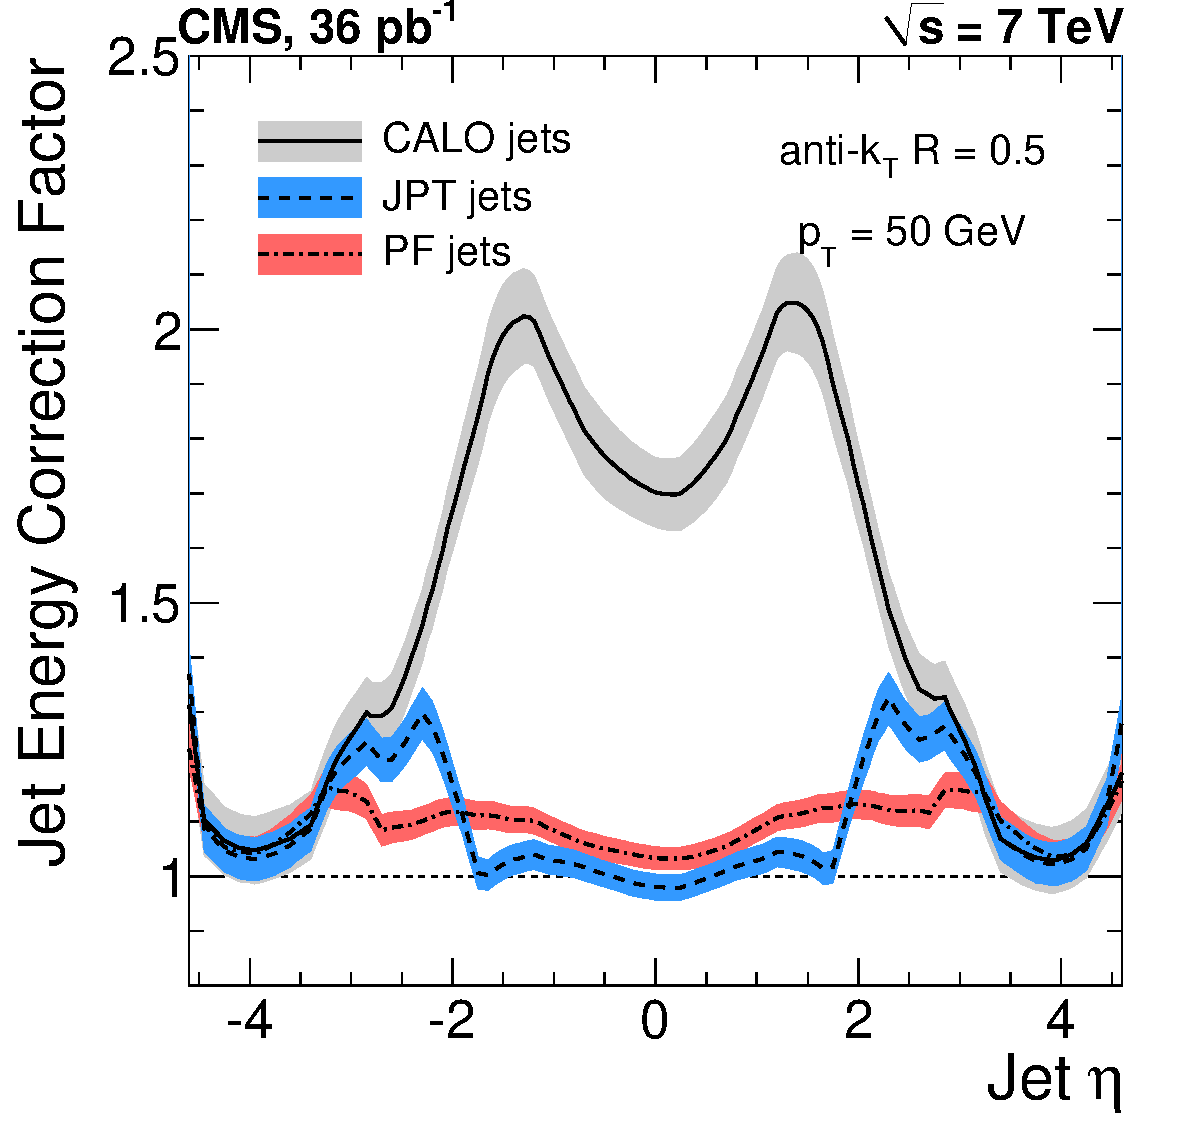
\includegraphics[width=0.45\textwidth]{Figures/JEC/JEC_vs_Eta_CorPt50}
    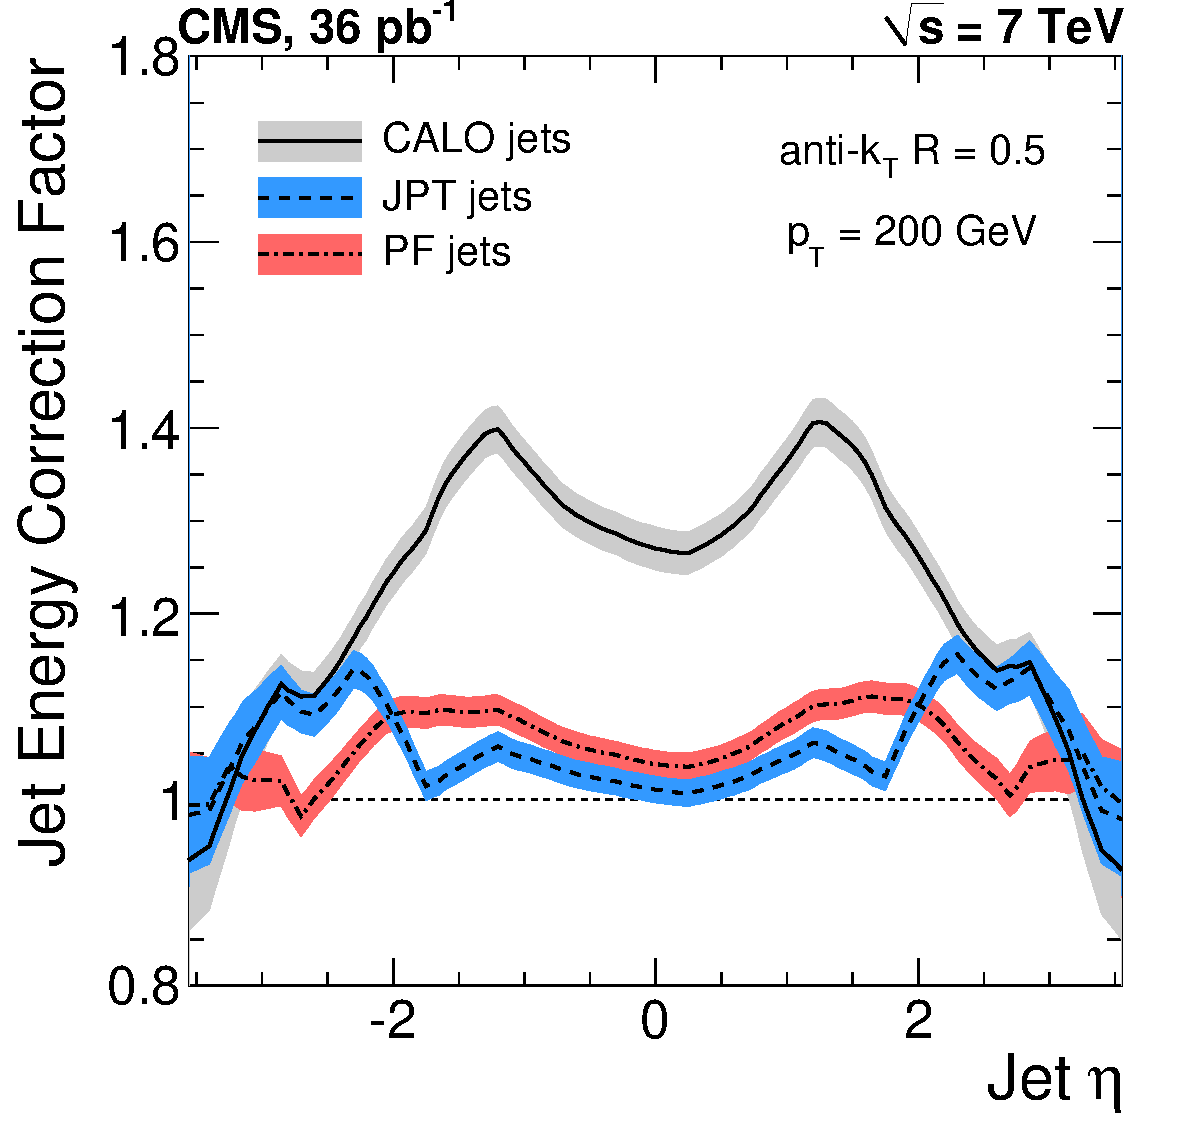
\includegraphics[width=0.45\textwidth]{Figures/JEC/JEC_vs_Eta_CorPt200}
    \caption{Total jet-energy-correction factor, as a function of jet $\eta$ for $\pt=50\GeV$ (left) and $\pt=200\GeV$ (right). The bands indicate the corresponding uncertainty.}
    \label{fig:finalJECvsEta}
  \end{center}
\end{figure}

\begin{figure}[ht!]
  \begin{center}
    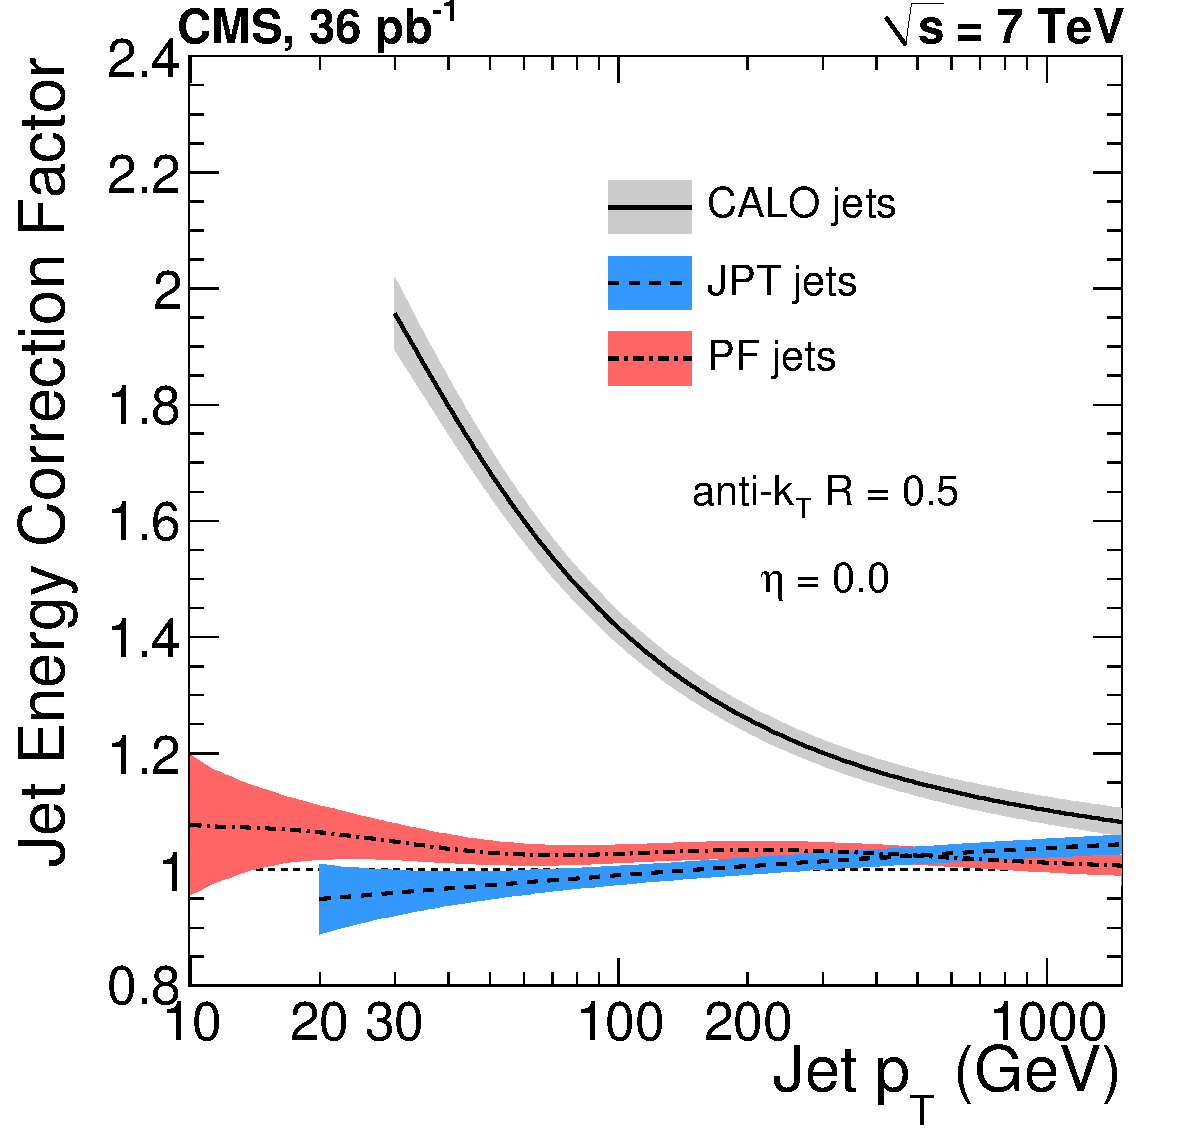
\includegraphics[width=0.45\textwidth]{Figures/JEC/JEC_vs_CorPt_eta0}
    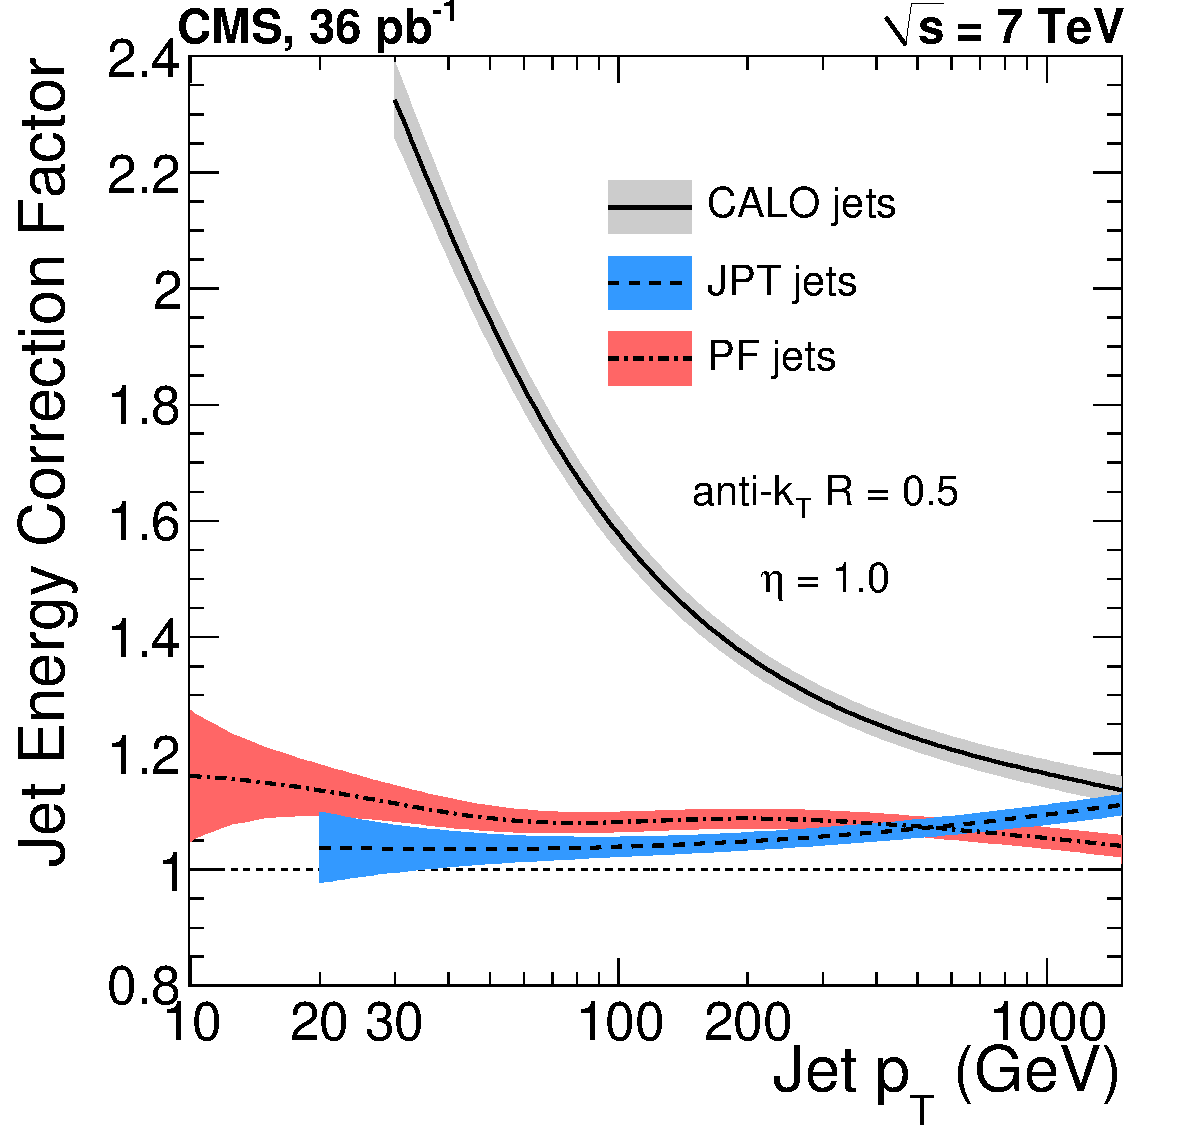
\includegraphics[width=0.45\textwidth]{Figures/JEC/JEC_vs_CorPt_eta10}
    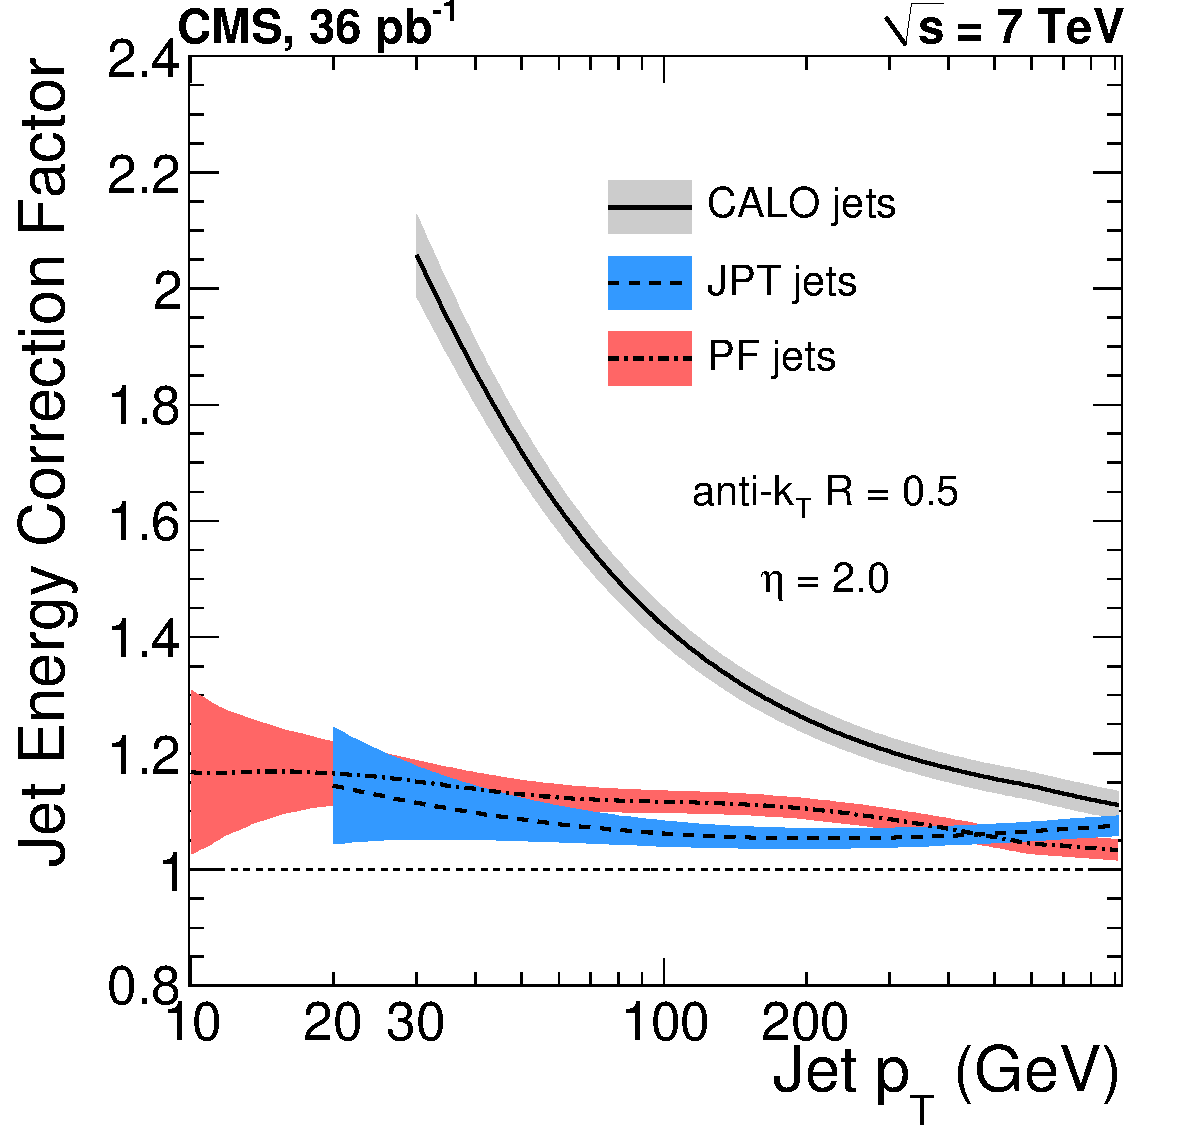
\includegraphics[width=0.45\textwidth]{Figures/JEC/JEC_vs_CorPt_eta20}
    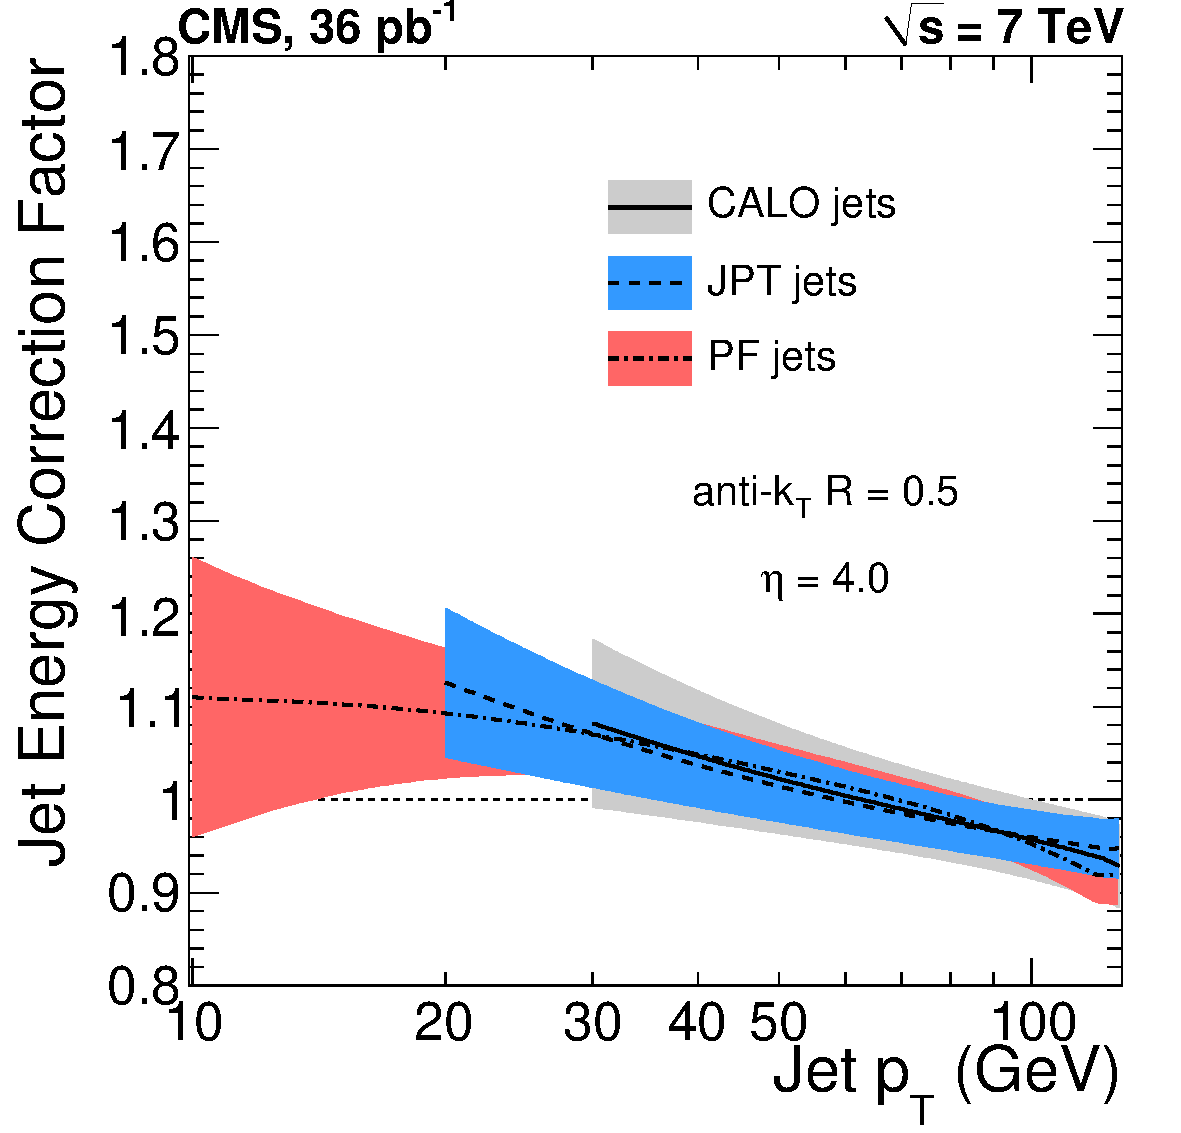
\includegraphics[width=0.45\textwidth]{Figures/JEC/JEC_vs_CorPt_eta40}
    \caption{Total jet-energy-correction factor, as a function of jet \pt for various $\eta$ values. The bands indicate the corresponding uncertainty.}
    \label{fig:finalJECvsPt}
  \end{center}
\end{figure}

\begin{figure}[ht!]
  \begin{center}
    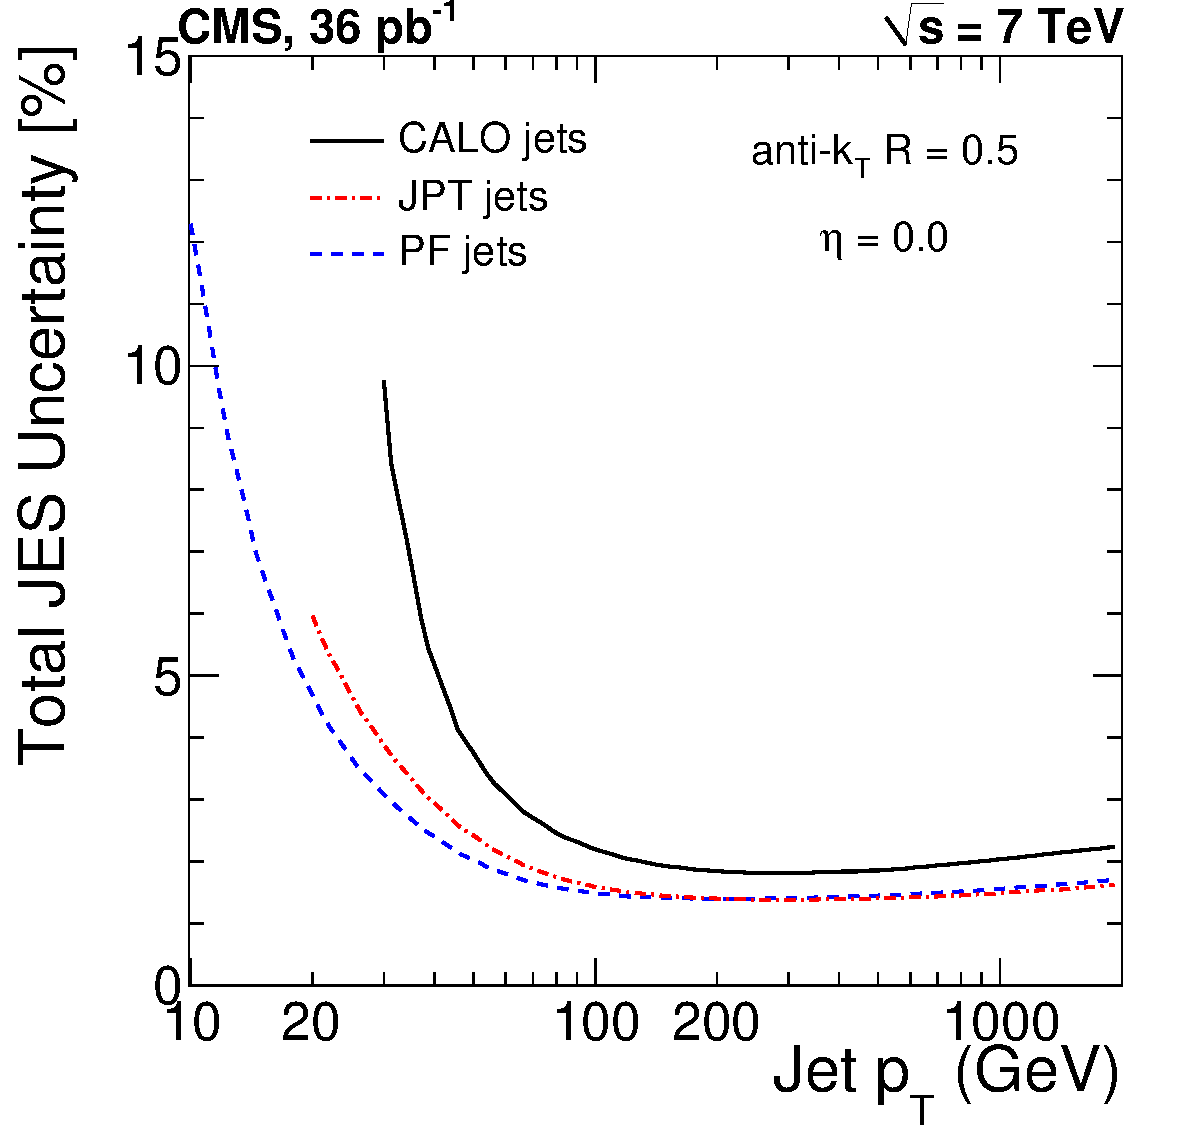
\includegraphics[width=0.45\textwidth]{Figures/JEC/Uncertainty_Eta0}
    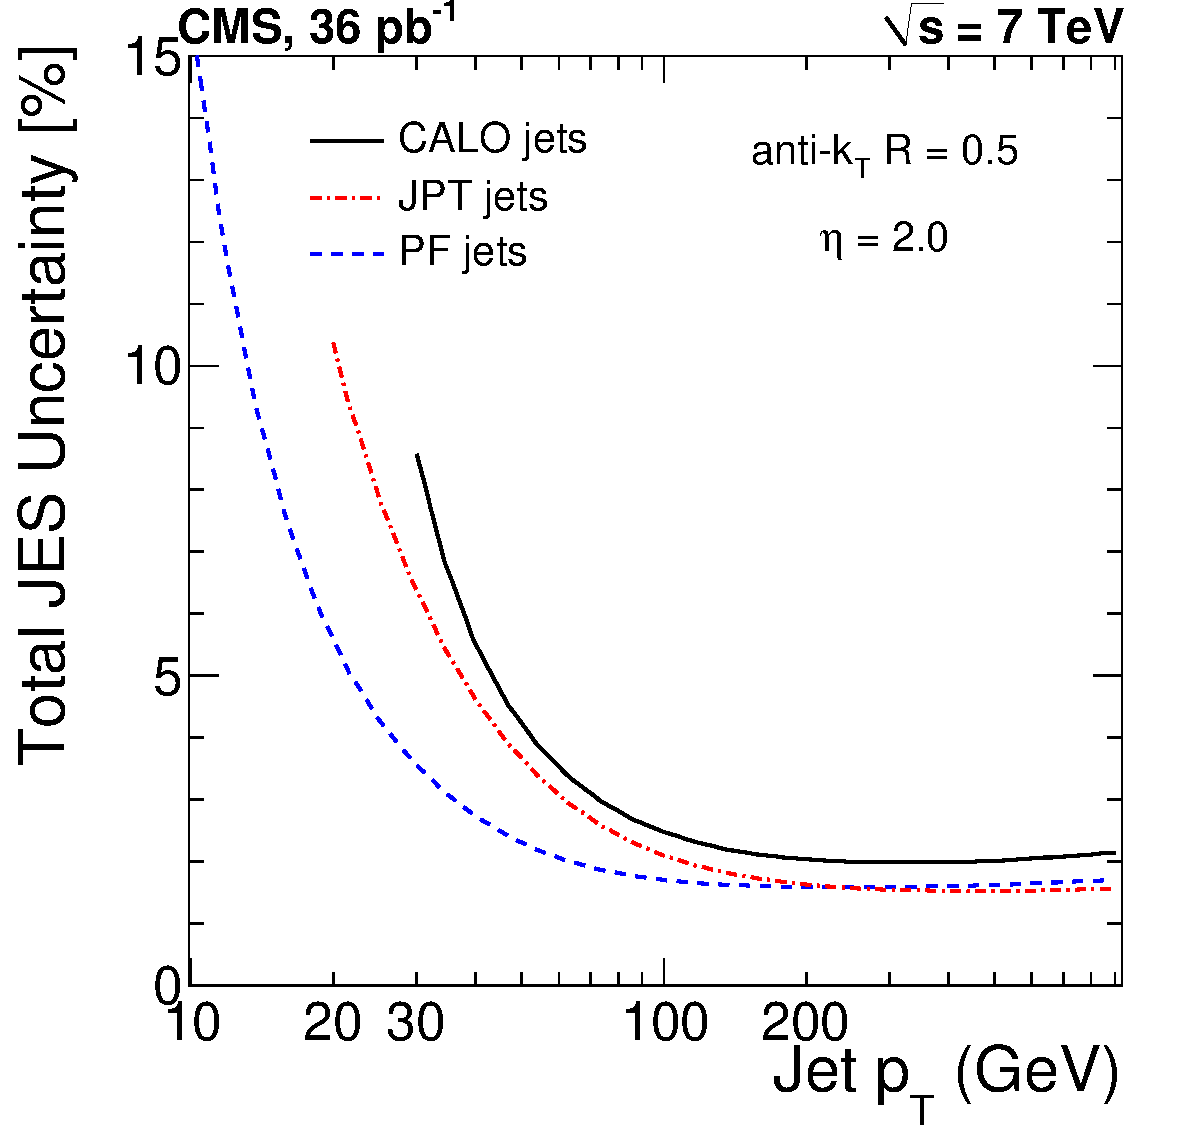
\includegraphics[width=0.45\textwidth]{Figures/JEC/Uncertainty_Eta20}
    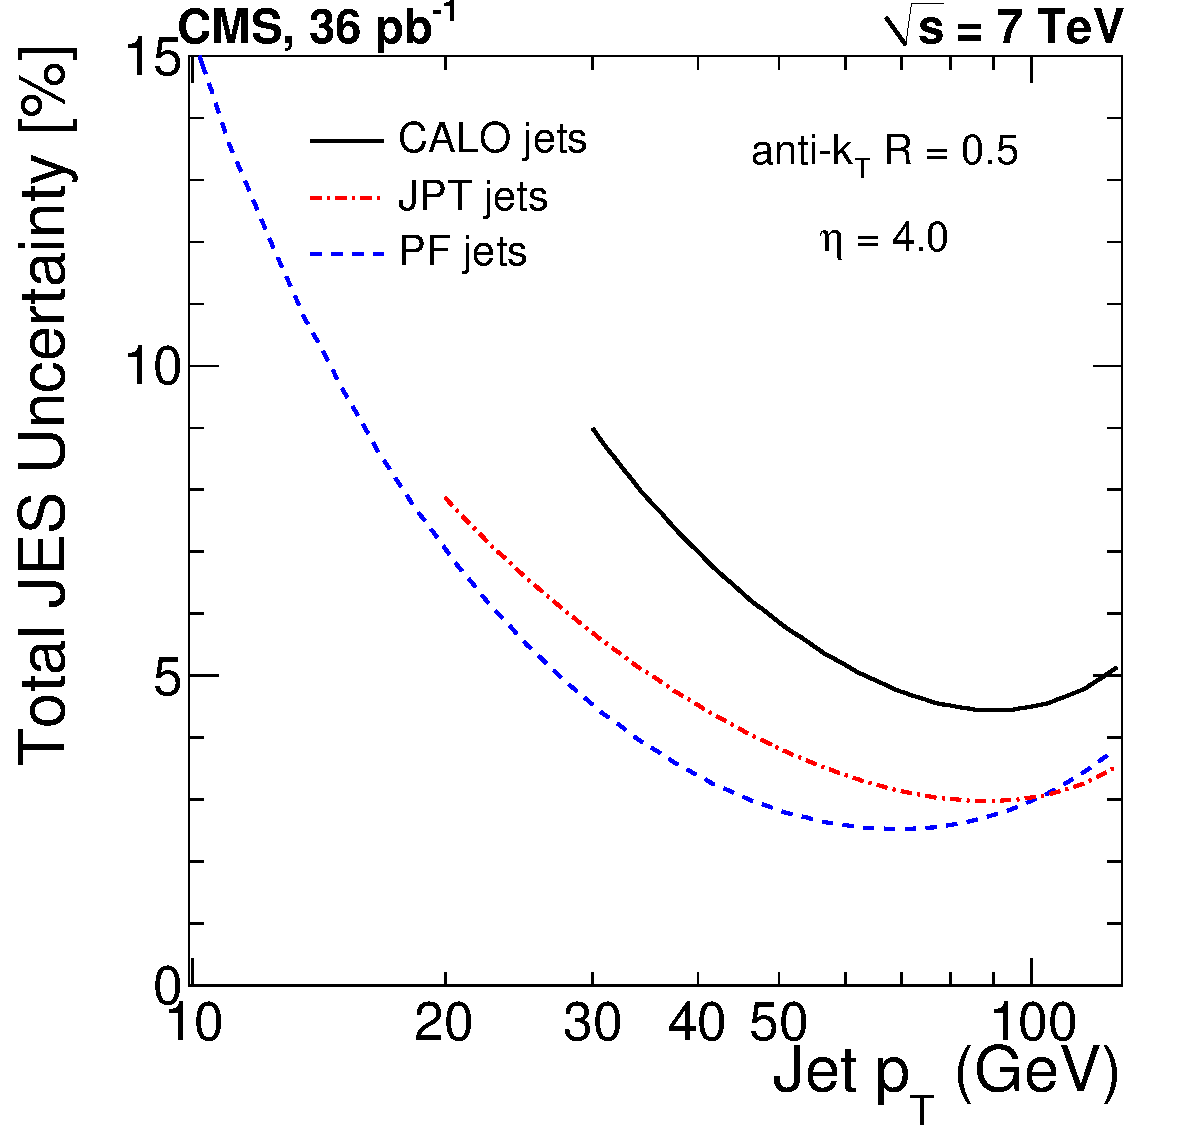
\includegraphics[width=0.45\textwidth]{Figures/JEC/Uncertainty_Eta40}
    \caption{Total jet-energy-scale uncertainty, as a function of jet \pt for various $\eta$ values.}
    \label{fig:finalUncvsPt}
  \end{center}
\end{figure}
